\documentclass[10pt, compress]{beamer}

\usetheme{m}

\usepackage{booktabs}
\usepackage[scale=2]{ccicons}
\usepackage{minted}

\usepgfplotslibrary{dateplot}

\usemintedstyle{trac}

\title{Estimation of Terrain Shape Using a Monocular Vision-based System}
\subtitle{Mid-Project Demonstration}
\date{\today}
\author{Connor Luke Goddard (clg11)}
\institute{Aberystwyth University}

\begin{document}

\maketitle

\begin{frame}[fragile]
  \frametitle{Introduction}

%  \textbf{Focus:} \\
%  \\ \vspace{0.5cm}
  
  \begin{block}{Focus}
    Investigation into a system capable of utilising a single, forward facing colour camera to provide an estimation into the shape of the environment terrain. 
  \end{block}
  
  \begin{block}{Potential areas of investigation}
    \begin{itemize}
  \item Detection of positive and negative obstacles.
  \item Detection of non-flat terrain (i.e. slopes).
  \item Estimation of the current speed.
  \item Estimation of the current rotation angle.
  \end{itemize}
  \end{block}

\end{frame}

%\section{Current Approach}

\begin{frame}[fragile]
  \frametitle{Current Approach}

  Approach focussed on the effects of \textbf{motion parallax}. \\ \vspace{0.5cm}
  
  \textbf{i.e.} Objects/features that are at a greater distance from the camera appear to  move less from frame-to-frame than those that are closer.
  
\begin{figure}[ht!]
\centering
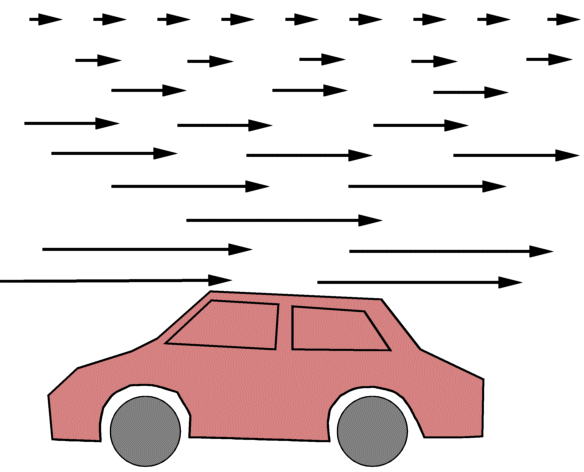
\includegraphics[scale=0.2]{motion_parallax.png}
    \caption{Typical example of motion parallax. \textbf{Courtesy}: \href{http://www.infovis.net}{http://www.infovis.net}.}
  \end{figure}
  

\end{frame}

\begin{frame}{Current Approach}

%Input: Two images with a set displacement between them (e.g. 10cm). \\

\textbf{Stage One} \\ \vspace{0.2cm}

Import two consecutive images, and convert from RGB (BGR in OpenCV) colour space to HSV.

\begin{figure}[ht!]
\centering
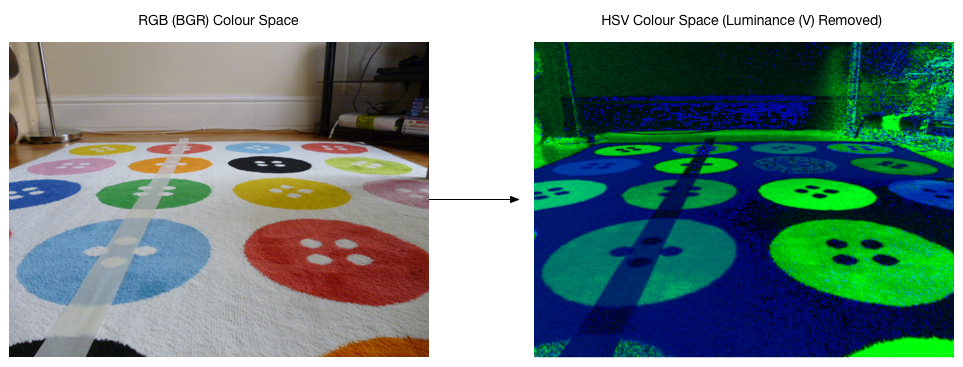
\includegraphics[scale=0.26]{rgb2hsv.png}
  \end{figure}
  
The 'V' channel is then removed in order to improve robustness to lighting changes between frames. 
\end{frame}

\begin{frame}{Current Approach}

\textbf{Stage Two} \\ \vspace{0.2cm}

Extract a percentage-width region of interest (ROI) from centre of first image.

\begin{figure}[ht!]
\centering
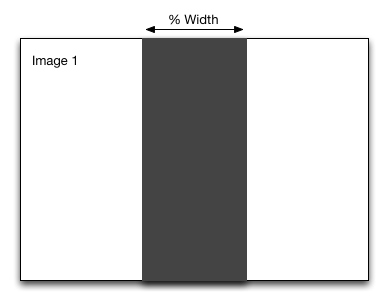
\includegraphics[scale=0.5]{stage1.png}
  \end{figure}
  
\end{frame}

\begin{frame}{Region-of-Interest}

\textbf{Why do we need to extract a ROI?} \\ \vspace{0.5cm}

\textbf{Focus-of-expansion}: Objects in images do not actually move in 1-dimension (i.e. straight down the image). \\ \vspace{0.2cm}

This effect is minimised towards the centre of the image.

\begin{figure}[ht!]
\centering
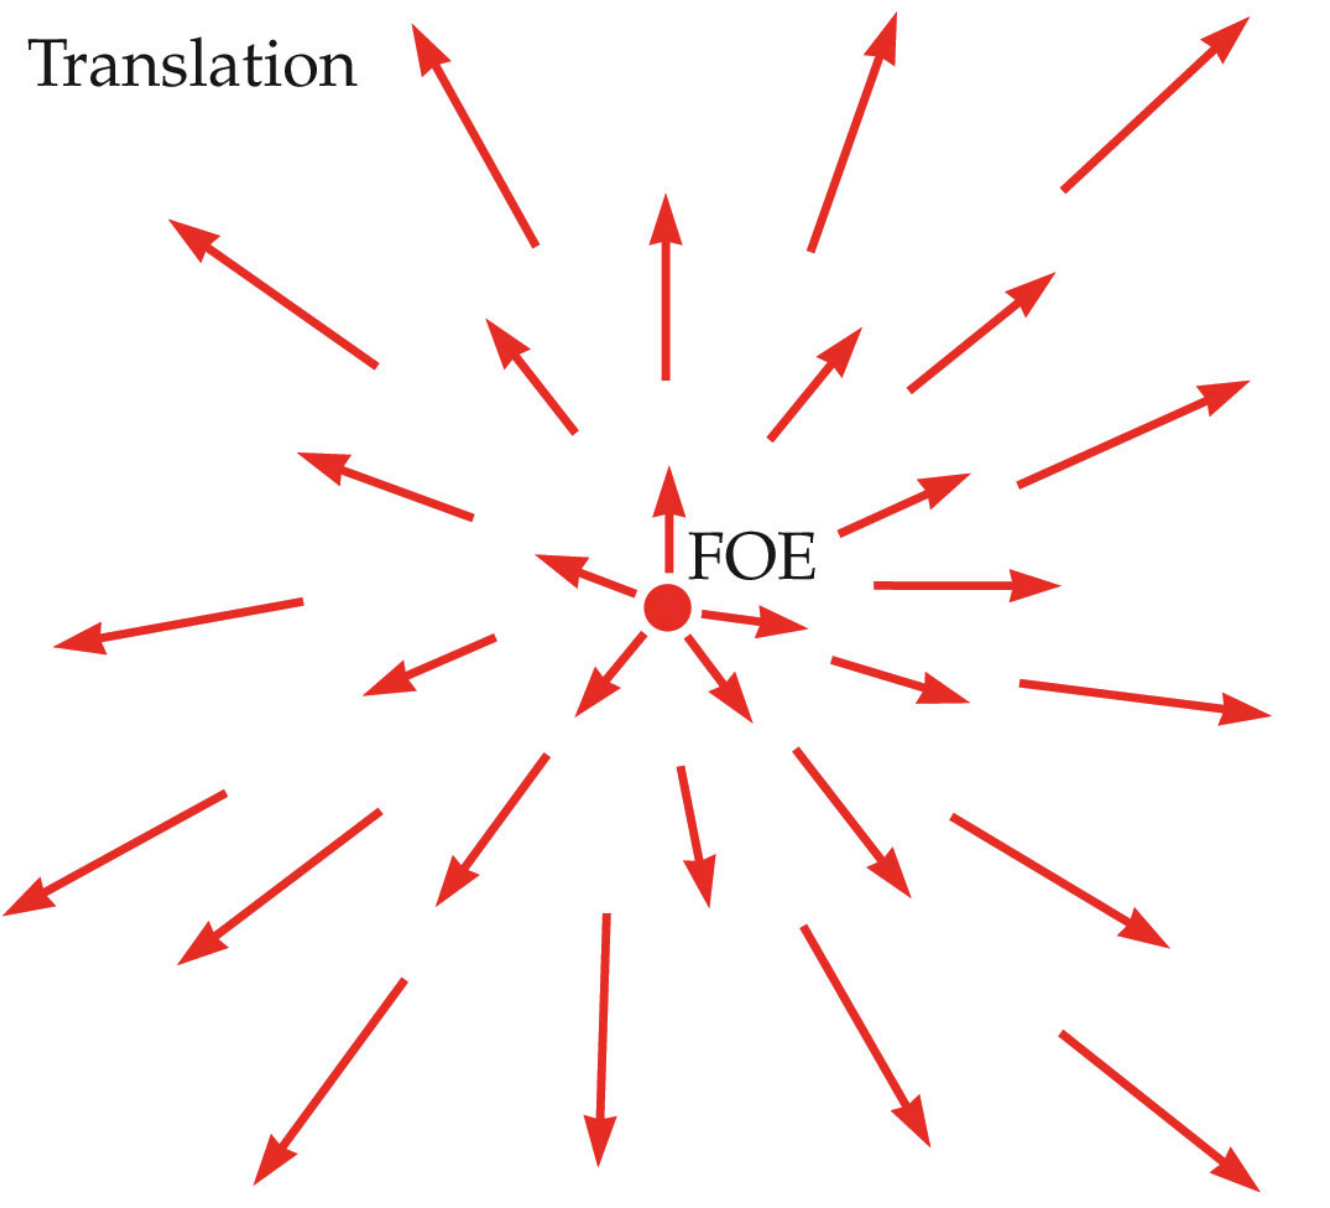
\includegraphics[scale=0.15]{foe.png}
\caption{\textbf{Courtesy:} J.Pillow, University of Texas}
  \end{figure}
  
\end{frame}

\begin{frame}{Current Approach}

\textbf{Stage Three} \\ \vspace{0.2cm}

Extract patches of a fixed size around each pixel within the extracted ROI.

\begin{figure}[ht!]
\centering
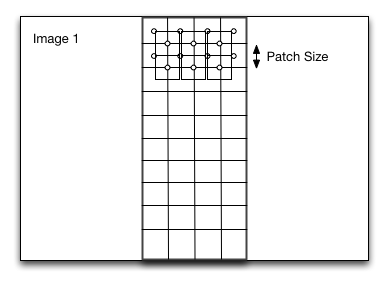
\includegraphics[scale=0.5]{stage2.png}
  \end{figure}
  
\end{frame}

\begin{frame}{Current Approach}

\textbf{Stage Four} \\ \vspace{0.2cm}

For each patch extracted from \emph{image one}, move down through a localised search window (column) in \emph{image two} searching for the best match against the template patch. 

\begin{figure}[ht!]
\centering
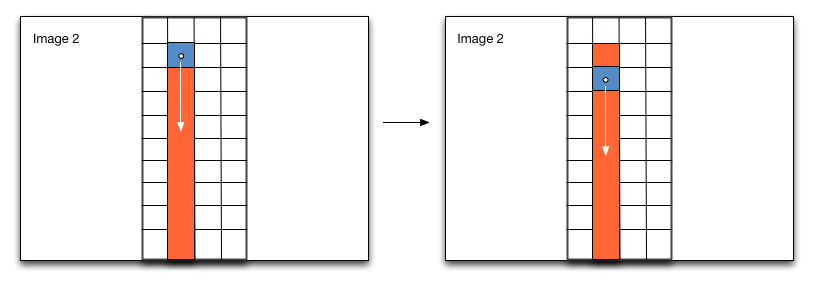
\includegraphics[scale=0.35]{stage3.png}
\end{figure}
  
\end{frame}

\begin{frame}{Current Approach}

\textbf{Stage Five} \\ \vspace{0.2cm}

Identify the patch within the localised search window that provides the ``best match" via correlation-based matching (e.g. Euclidean Distance, SSD or Correlation coefficient). 

\begin{figure}[ht!]
\centering
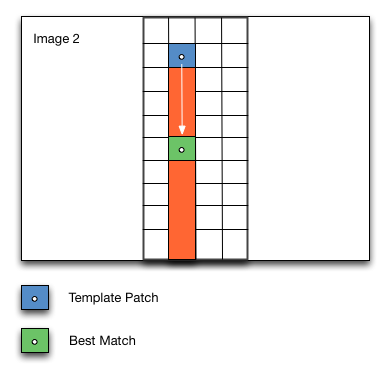
\includegraphics[scale=0.35]{stage4.png}
\end{figure}

\end{frame}

\begin{frame}{Current Approach}

\textbf{Stage Six} \\ \vspace{0.2cm}

Average all measured displacements for each pixel along a given row.

\begin{figure}[ht!]
\centering
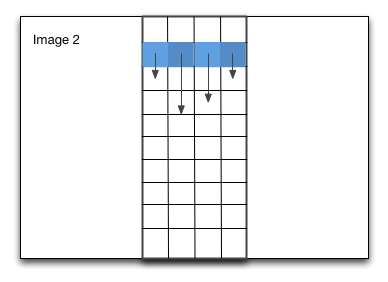
\includegraphics[scale=0.4]{stage5.png}
\end{figure}

Outliers are removed by ignoring any displacements that lie outside of (2 x Standard Deviation) of the mean.

\end{frame}

\begin{frame}{Current Approach}

\textbf{Repeat Stages 1-6} \\ \vspace{0.2cm}

Repeat stages 1-6 for an entire collection of ``calibration" images taken of \emph{flat, unobstructed} terrain.

\begin{figure}[ht!]
\centering
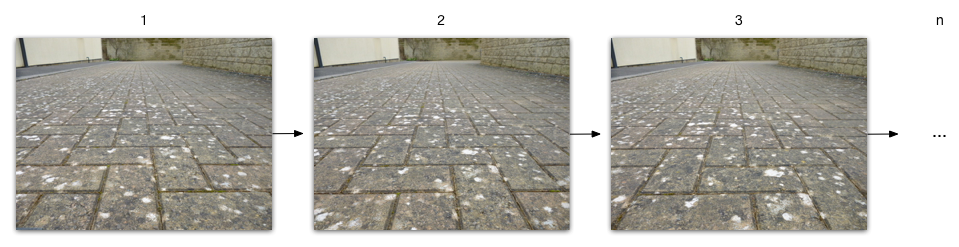
\includegraphics[scale=0.3]{calibimages.png}
\end{figure}

\end{frame}

\begin{frame}{Current Approach}

\textbf{Stage Seven} \\ \vspace{0.2cm}

Plot the \emph{average displacement} for each ROI row, calculated from the displacements recorded over all calibration images.

\begin{figure}[ht!]
\centering
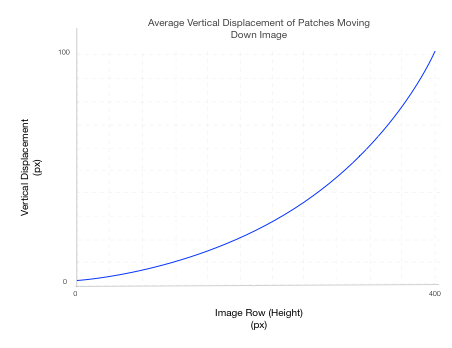
\includegraphics[scale=0.45]{graph.png}
\end{figure}

\end{frame}



\begin{frame}{Results}

Generally ``mixed" results at this stage. \\ \vspace{0.5cm}

From the results obtained, we have learned:

\begin{enumerate}
  \item It is possible to potentially establish a relationship between row height in an image, and average downwards pixel displacement.
  \item The current approach to appearance-based tracking using multiple ``small" patches \textbf{does not work well} for many typical terrain conditions (i.e. outside). 
\end{enumerate}

\end{frame}

\begin{frame}{Results: Example 1}

\begin{columns}[T] % align columns
\begin{column}{.48\textwidth}

\textbf{Input Collection:}

\begin{figure}[ht!]
\centering
\vspace{0.3cm}
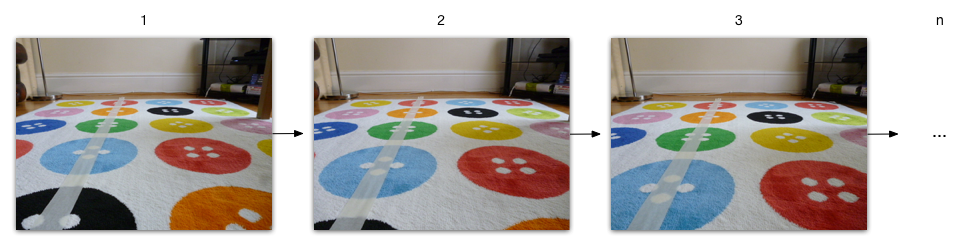
\includegraphics[scale=0.18]{calibimages_good.png}
\end{figure}

\end{column}%
\hfill%
\begin{column}{.48\textwidth}

\textbf{Result:}

\begin{figure}[ht!]
\centering
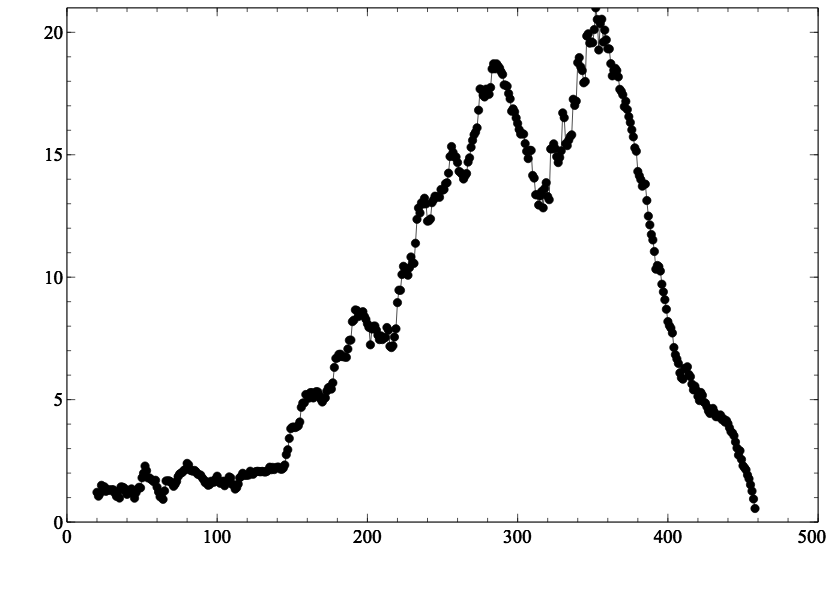
\includegraphics[scale=0.22]{flat_10cm_results.png}
\end{figure}

\end{column}%
\end{columns}

\end{frame}

\begin{frame}{Results: Example 2}

\begin{columns}[T] % align columns
\begin{column}{.48\textwidth}

\textbf{Input Collection:}

\begin{figure}[ht!]
\centering
\vspace{0.3cm}
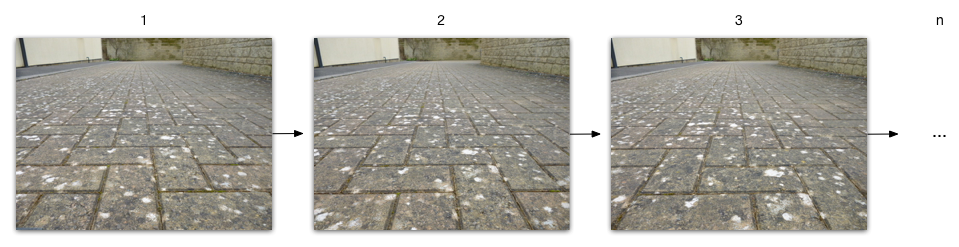
\includegraphics[scale=0.18]{calibimages.png}
\end{figure}

\end{column}%
\hfill%
\begin{column}{.48\textwidth}

\textbf{Result:}
\begin{figure}[ht!]
\centering
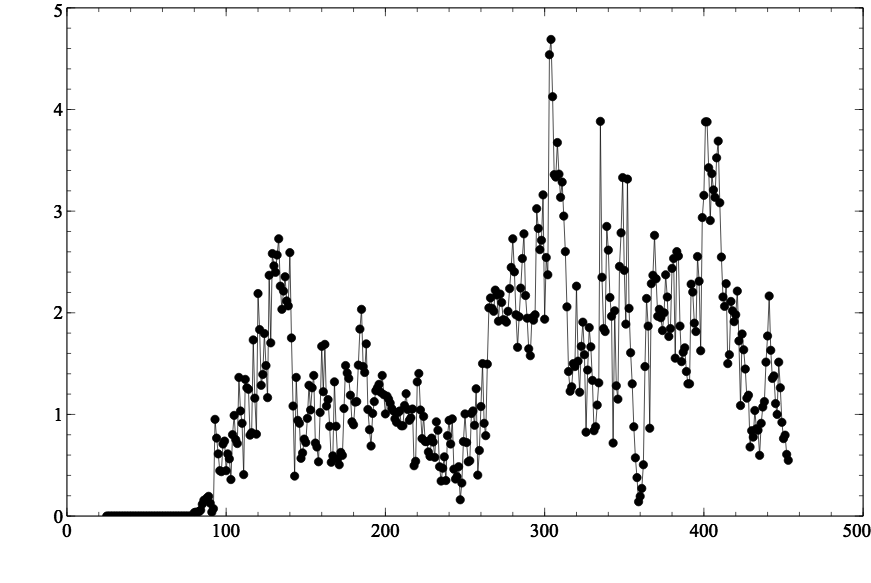
\includegraphics[scale=0.22]{wiltshire_outside_10cm.png}
\end{figure}

\end{column}%
\end{columns}

\end{frame}

\begin{frame}{Next Steps}

Plan is to move away from multiple small patches instead adopting a single, larger patch to represent a single row. \\ \vspace{0.5cm}

Template patch will be scaled relative to its centre as the search moves down the image. This is to account for perspective distortion (\textbf{i.e.} objects becoming larger as they move closer to the camera).

\begin{figure}[ht!]
\centering
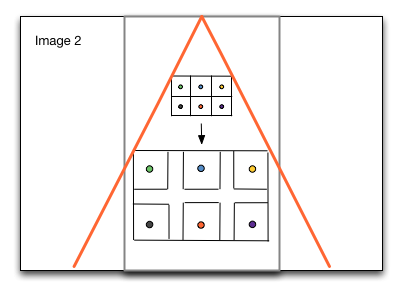
\includegraphics[scale=0.4]{scaling.png}
\end{figure}
	
\end{frame}

\begin{frame}{Project Management}

Project is adopting a SCRUM-based approach to project management. \\ \vspace{0.2cm}

\begin{itemize}
	\item \textbf{Releases} - Major feature sets (e.g. work up to mid-project demo)
	\item \textbf{Sprints} - Weekly time-boxed portion of work effort.
	\item \textbf{Sprint Review \& Retrospectives} - Conducted as part of weekly project meeting with tutor. 
\end{itemize}


\textbf{Tools:} \textit{Github Issues} with \textit{\href{http://waffle.io}{Waffle.io}} (KANBAN), \textit{\href{http://burndown.io/}{Burndown.io}} (Burndown charts).
	
\end{frame}

\begin{frame}{Project Management}

\begin{figure}[ht!]
\centering
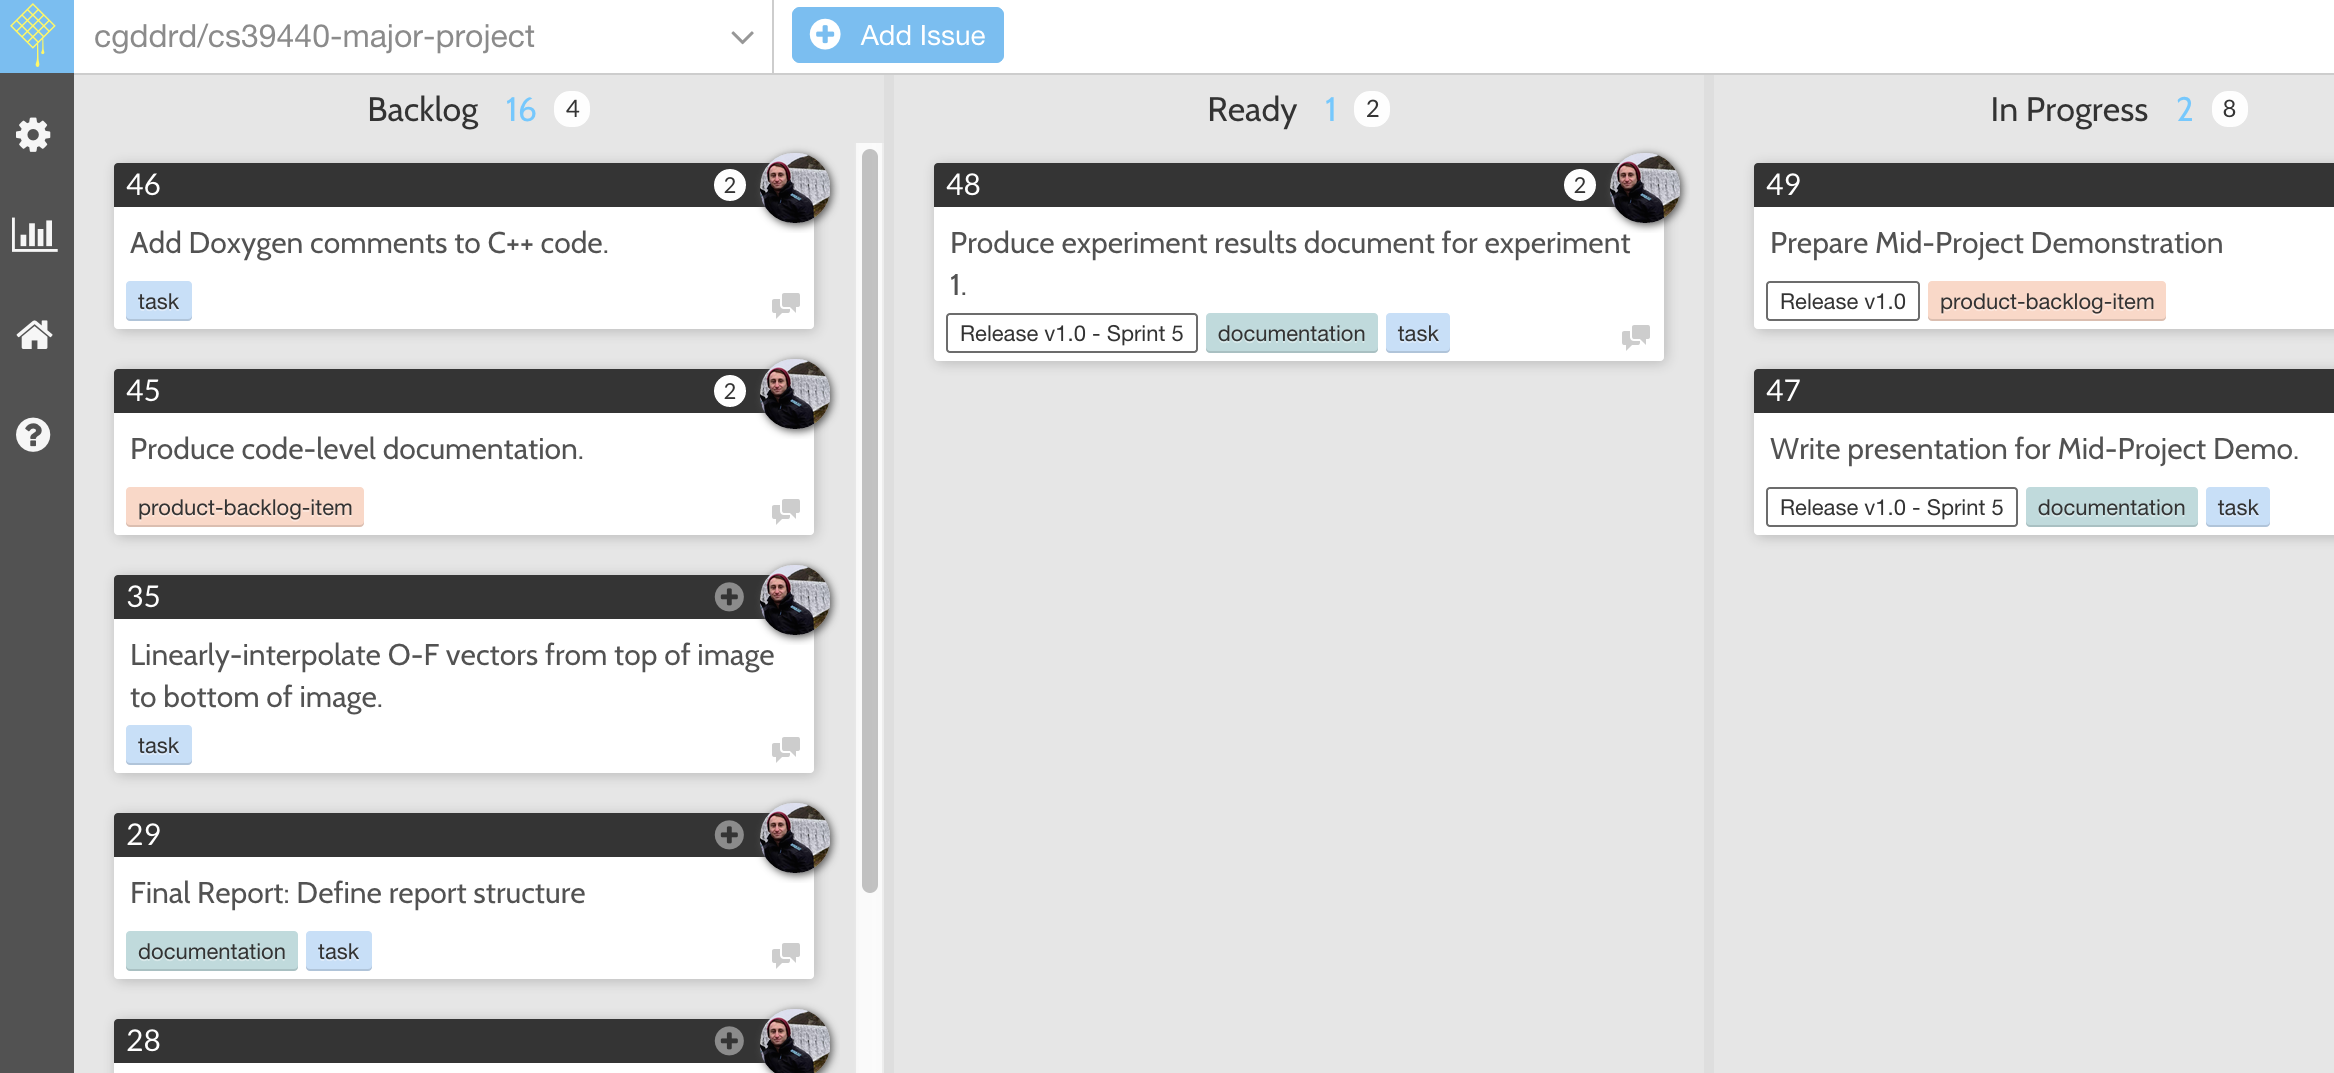
\includegraphics[scale=0.12]{waffle.png}
\caption{Waffle.io KANBAN board interface to Github Issues.}
\end{figure}

\begin{figure}[ht!]
\centering
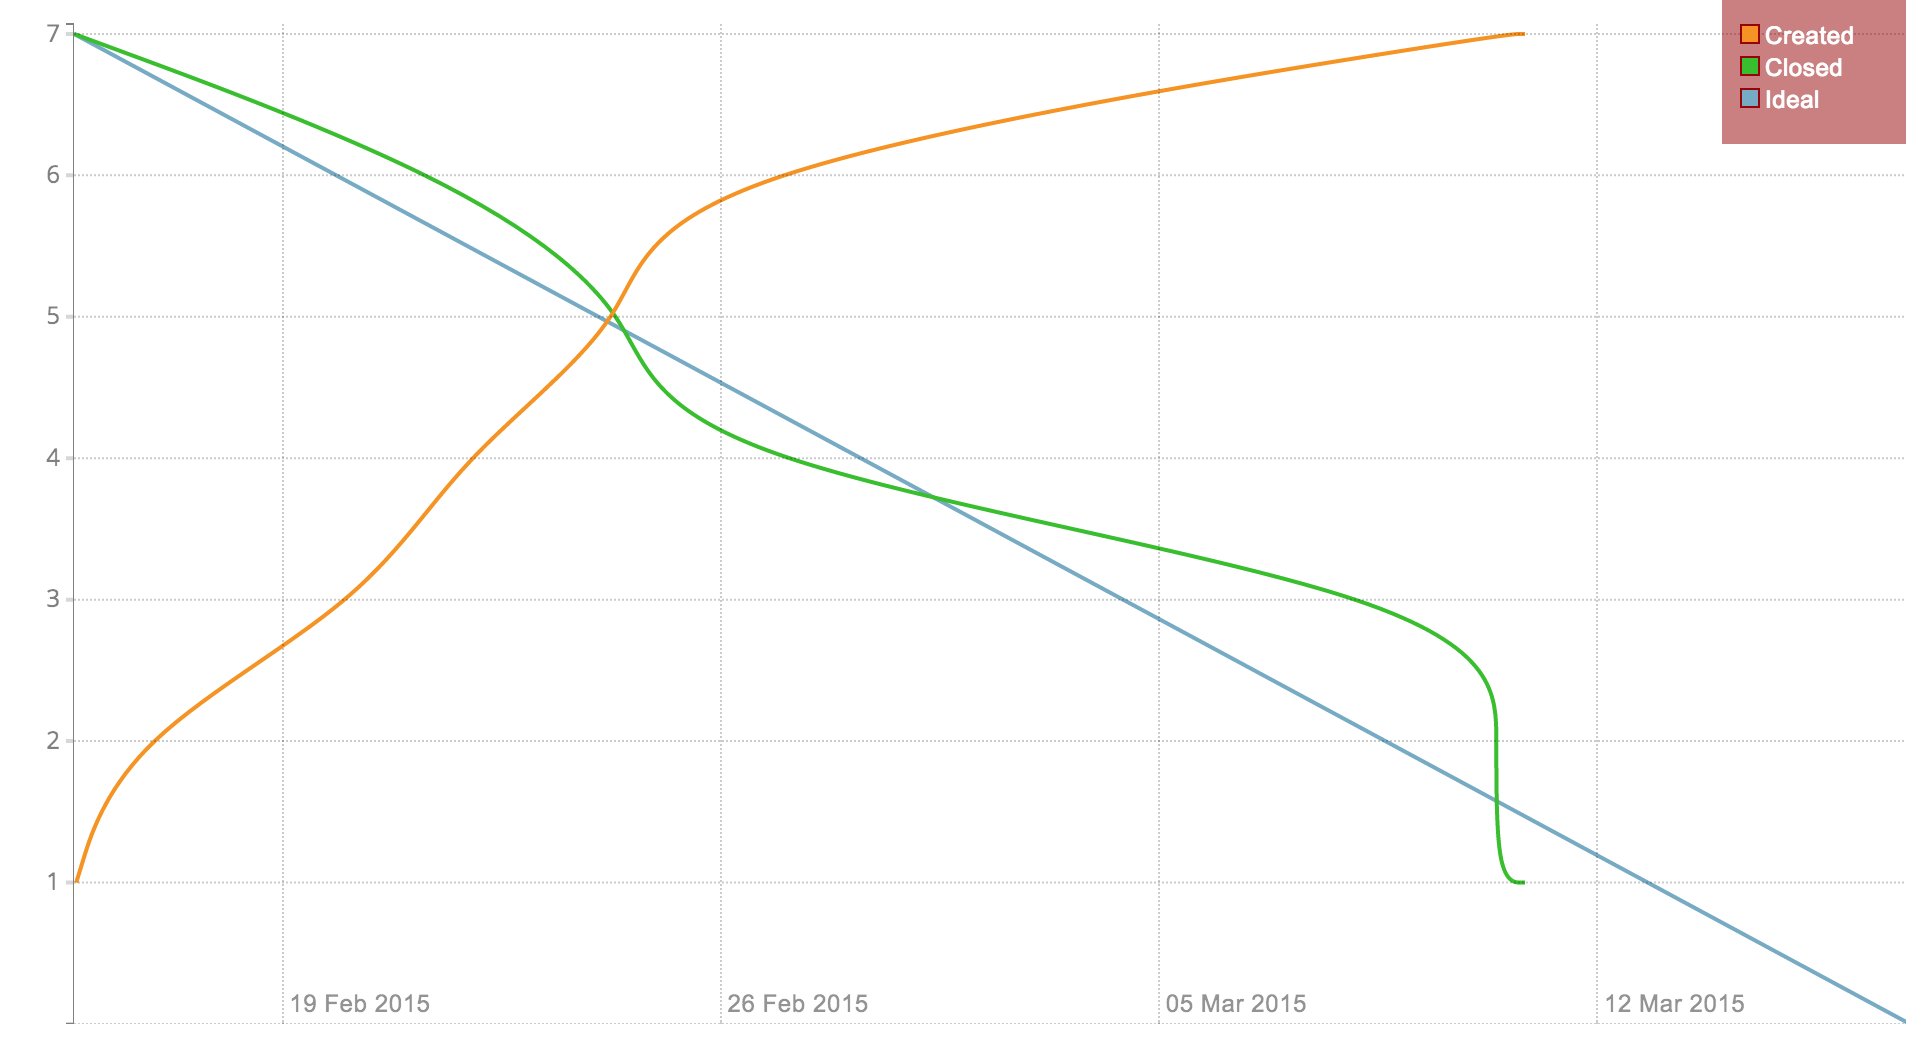
\includegraphics[scale=0.12]{burndown.png}
\caption{Burndown chart for Release v1.0. \textbf{Courtesy:} \href{http://burndown.io}{http://burndown.io}}
\end{figure}

\end{frame}

\plain{Any Questions? \\ \vspace{0.2cm} \footnotesize{Slide Design: Matthias Vogelgesang - (\href{https://github.com/matze/mtheme}{Github})}}

\end{document}
